\subsection{Tablice figur}
\label{subsec:tablice-figur}

\subsubsection{Opis zagadnienia}
Istotnym z punktu widzenia heurystyki silnika jest prawidłowa ocena informacji na planszy.
Ograniczona wiedza, jedynie co do ilości figur na planszy, była niewystarczająca, aby móc prowadzić rozgrywkę na odpowiednio wysokim poziomie.

Wraz z rozwojem strategii szachowych gracze wypracowali szereg schematów, które ułatwiają im podejmowanie decyzji, niezależnie od konkretnej sytuacji na planszy.
Są nimi między innymi: zajęcie centralnych pól przez pionki, nierozwijanie skoczka na skrajne pola planszy, czy pozycjonowanie wież na otwartych liniach i wierszach pionów przeciwnika.

\subsubsection{Implementacja}
Implementacja każdego z powyższych, jak i wielu innych reguł mogłaby okazać się czasochłonna i złożona obliczeniowo.
Zdecydowano się zatem na zastosowanie tablic figur, które można rozumieć jako mapy cieplne, reprezentujące korzystność umieszczenia figury na danym polu.
Dla każdego typu bierki ($2*6$) stworzono tablicę 64 elementową określającą wartości, odnośnie do tego, jak korzystne jest umieszczenie figury na danym polu.
Zastosowano się na nie tworzenie własnych tablic, a zastosowanie gotowych, dostępnych na forum tworzenia silników szachowych. \cite*{wiki-tablica-figur}

\begin{figure}[ht]
    \centering
    \begin{tabular}{@{}ll@{}}
        a) & b) \\
        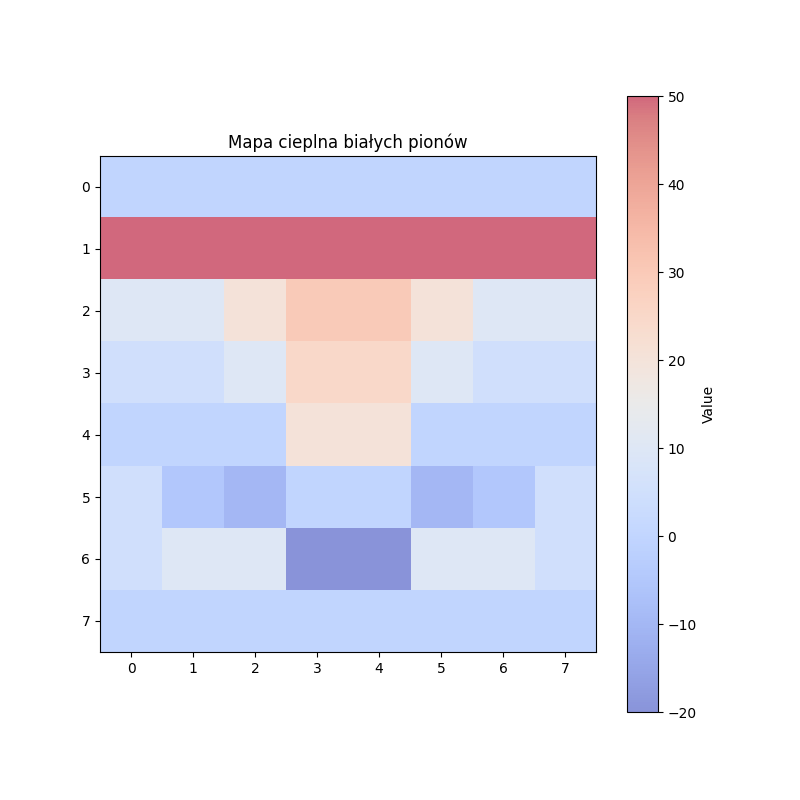
\includegraphics[width=0.5\textwidth]{rozdzialy/rozdzial02/2_ulepszenia_oceny/rysunki/bialePiony}
        &
        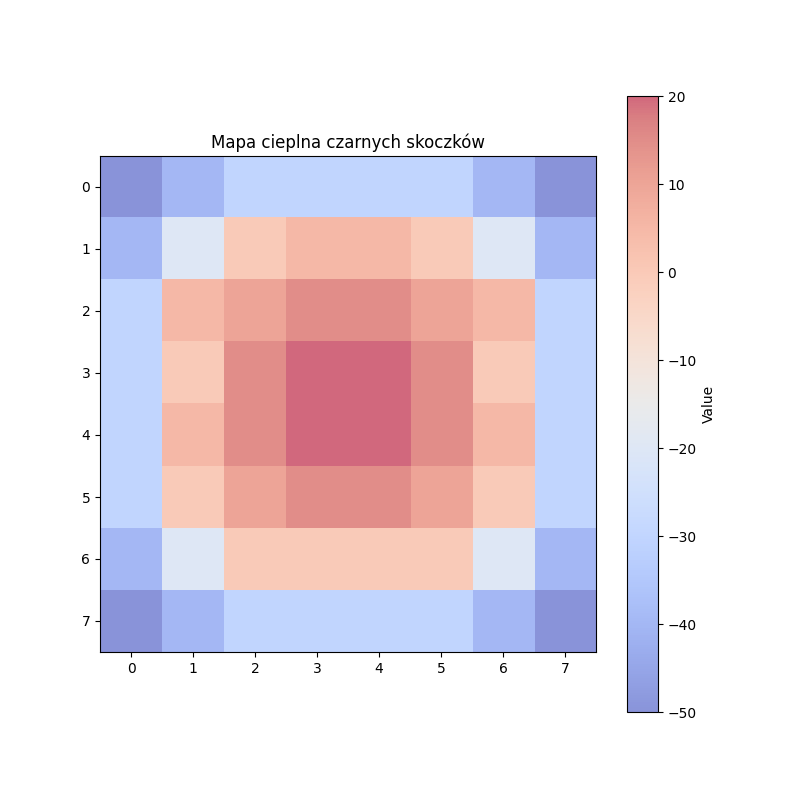
\includegraphics[width=0.5\textwidth]{rozdzialy/rozdzial02/2_ulepszenia_oceny/rysunki/czarneSkoczki}
    \end{tabular}
    \caption{Przykładowe tablice cieplne bierek: a) białych pionów, b) czarnych skoczków}
    \label{fig: tablice-figur}
\end{figure}

Rezultatem zastosowania tablic figur stał się silnik, który w odczuciu autora znacznie lepiej \enquote{rozumiał} pozycję na planszy.